\documentclass[aspectratio=43,fleqn]{beamer}
\usetheme[
%%% options passed to the outer theme
%    hidetitle,           % hide the (short) title in the sidebar
    hideauthor,          % hide the (short) author in the sidebar
%    hideinstitute,       % hide the (short) institute in the bottom of the sidebar
%    shownavsym,          % show the navigation symbols
%    width=2cm,           % width of the sidebar (default is 2 cm)
%    hideothersubsections,% hide all subsections but the subsections in the current section
%    hideallsubsections,  % hide all subsections
    left               % right of left position of sidebar (default is right)
%%% options passed to the color theme
%    lightheaderbg,       % use a light header background
  ]{AAUsidebar}

% If you want to change the colors of the various elements in the theme, edit and uncomment the following lines
% Change the bar and sidebar colors:
%\setbeamercolor{AAUsidebar}{fg=red!20,bg=red}
%\setbeamercolor{sidebar}{bg=red!20}
% Change the color of the structural elements:
%\setbeamercolor{structure}{fg=red}
% Change the frame title text color:
\definecolor{titleback}{RGB}{14,81,149}
\setbeamercolor{frametitle}{bg=titleback}
% Change the normal text color background:
%\setbeamercolor{normal text}{bg=gray!10}
% ... and you can of course change a lot more - see the beamer user manual.

\usepackage{xeCJK}
\usepackage{amsmath}
\usepackage{amsfonts}
\usepackage{bm}%bold form in math environment
 %\sideset{}{}\sum  求和符号左上角,右上角添加标记
\usepackage{graphicx}
\usepackage{wrapfig}
\usepackage{subfigure}%多图共用caption
\usepackage{fontspec}
\usepackage{xunicode}
\usepackage{multicol}
\usepackage{amssymb}
\usepackage{amsthm}
\usepackage[english]{babel}
\usepackage[T1]{fontenc}
\usepackage{textcomp}
\usepackage{listings} %codes support
\usepackage{xcolor}
% Or whatever. Note that the encoding and the font should match. If T1
% does not look nice, try deleting the line with the fontenc.
\usepackage{helvet}

\XeTeXlinebreaklocale "zh"
\setCJKmainfont[BoldFont=SimHei]{Microsoft YaHei}
\setCJKmonofont{SimSun}
\setCJKfamilyfont{yahei}{Microsoft YaHei}
\newcommand{\yahei}{\CJKfamily{yahei}} 
\setCJKfamilyfont{hei}{SimHei}
\newcommand{\heiti}{\CJKfamily{hei}}
\setCJKfamilyfont{zs}{STZhongsong}
\newcommand{\zhongsong}{\CJKfamily{zs}}
\setCJKfamilyfont{kai}{KaiTi}
\newcommand{\kaishu}{\CJKfamily{kai}} 
\newfontfamily\codefont{Source Code Pro}

\setlength{\baselineskip}{0em}
\newcommand{\chuhao}{\fontsize{42pt}{\baselineskip}\selectfont}     %初号  
\newcommand{\xiaochuhao}{\fontsize{36pt}{\baselineskip}\selectfont} %小初号  
\newcommand{\yihao}{\fontsize{28pt}{\baselineskip}\selectfont}      %一号  
\newcommand{\erhao}{\fontsize{21pt}{\baselineskip}\selectfont}      %二号  
\newcommand{\xiaoerhao}{\fontsize{18pt}{\baselineskip}\selectfont}  %小二号  
\newcommand{\sanhao}{\fontsize{15.75pt}{\baselineskip}\selectfont}  %三号  
\newcommand{\sihao}{\fontsize{14pt}{18pt}\selectfont}%     四号  
\newcommand{\xiaosihao}{\fontsize{12pt}{24pt}\selectfont}  %小四号  
\newcommand{\wuhao}{\fontsize{10.5pt}{\baselineskip}\selectfont}    %五号  
\newcommand{\xiaowuhao}{\fontsize{9pt}{\baselineskip}\selectfont}   %小五号  
\newcommand{\liuhao}{\fontsize{6.5pt}{\baselineskip}\selectfont}  %六号  
\newcommand{\qihao}{\fontsize{5.25pt}{\baselineskip}\selectfont}    %七

\renewcommand{\figurename}{\heiti 图}
\renewcommand{\thefigure}{\arabic{section}--\arabic{figure}}
\renewcommand{\tablename}{\heiti 表}
\renewcommand{\thetable}{\arabic{section}--\arabic{table}}
% colored hyperlinks
\newcommand{\chref}[2]{%
  \href{#1}{{\usebeamercolor[bg]{AAUsidebar}#2}}%
}

\title[基于Android的ECG监测与记录应用实现]% optional, use only with long paper titles
{基于Android的ECG监测与记录应用实现}

\subtitle{本科生毕业论文答辩}  % could also be a conference name
\date{\today}

\author[某某某] % optional, use only with lots of authors
{
  答辩人:某某某\\
  指导教师:某某某
}
% - Give the names in the same order as they appear in the paper.
% - Use the \inst{?} command only if the authors have different
%   affiliation. See the beamer manual for an example

\institute[
%  {\includegraphics[scale=0.2]{aau_segl}}\\ %insert a company, department or university logo
  华中科技大学\\
  光电信息学院
] % optional - is placed in the bottom of the sidebar on every slide
{% is placed on the title page
  光学与电子信息学院\\
  华中科技大学
  %there must be an empty line above this line - otherwise some unwanted space is added between the university and the country (I do not know why;( )
}


% specify a logo on the titlepage (you can specify additional logos an include them in 
% institute command below
\pgfdeclareimage[height=1.5cm]{titlepagelogo}{pics/aau_logo_new.png} % placed on the title page
%\pgfdeclareimage[height=1.5cm]{titlepagelogo2}{graphics/aau_logo_new} % placed on the title page
\titlegraphic{% is placed on the bottom of the title page
  \pgfuseimage{titlepagelogo}
%  \hspace{1cm}\pgfuseimage{titlepagelogo2}
}


\begin{document}
%%%%%%%%%%%%%%%%%%%%%%%%%%%%%%%code support%%%%%%%%%%%%%%%%%%%%%%%%%%%%
\lstset{basicstyle=\codefont\fontsize{8pt}{7.5pt}\selectfont,breaklines=true,numbers=left,numberstyle=\codefont\tiny,keywordstyle=\color{blue!70},commentstyle=\color{red!50!green!50!blue!50},frame=shadowbox, rulesepcolor=\color{red!20!green!20!blue!20},escapeinside=``,xleftmargin=2em,xrightmargin=2em, aboveskip=1em}
%%%%%%%%%%%%%%%%%%%%%%%%%%%%%%%code support end%%%%%%%%%%%%%%%%%%%%%%%%

{\aauwavesbg
\begin{frame}[plain,noframenumbering]
\titlepage
\end{frame}}

\begin{frame}{目录}{}
\tableofcontents
\end{frame}

\section{研究背景}
\begin{frame}{研究背景}{}
  \begin{itemize}
    \item<1-> Android平台覆盖面广、接口丰富、易于开发
    \item<2-> ECG监测设备的小型化和智能化
    \item<3-> 相关研究对两者的结合做出了尝试
    \item<4-> 相关研究显示不够友好、无法提供精确的数值
  \end{itemize}
\end{frame}

\section{研究成果}
\subsection{显示方法的改进}
\begin{frame}{研究成果}{适应波形 可交互的显示方法}
	\begin{columns}
		\column{0.5\textwidth}
			\only<1>
			{\begin{figure}[ht]
			\begin{center}
				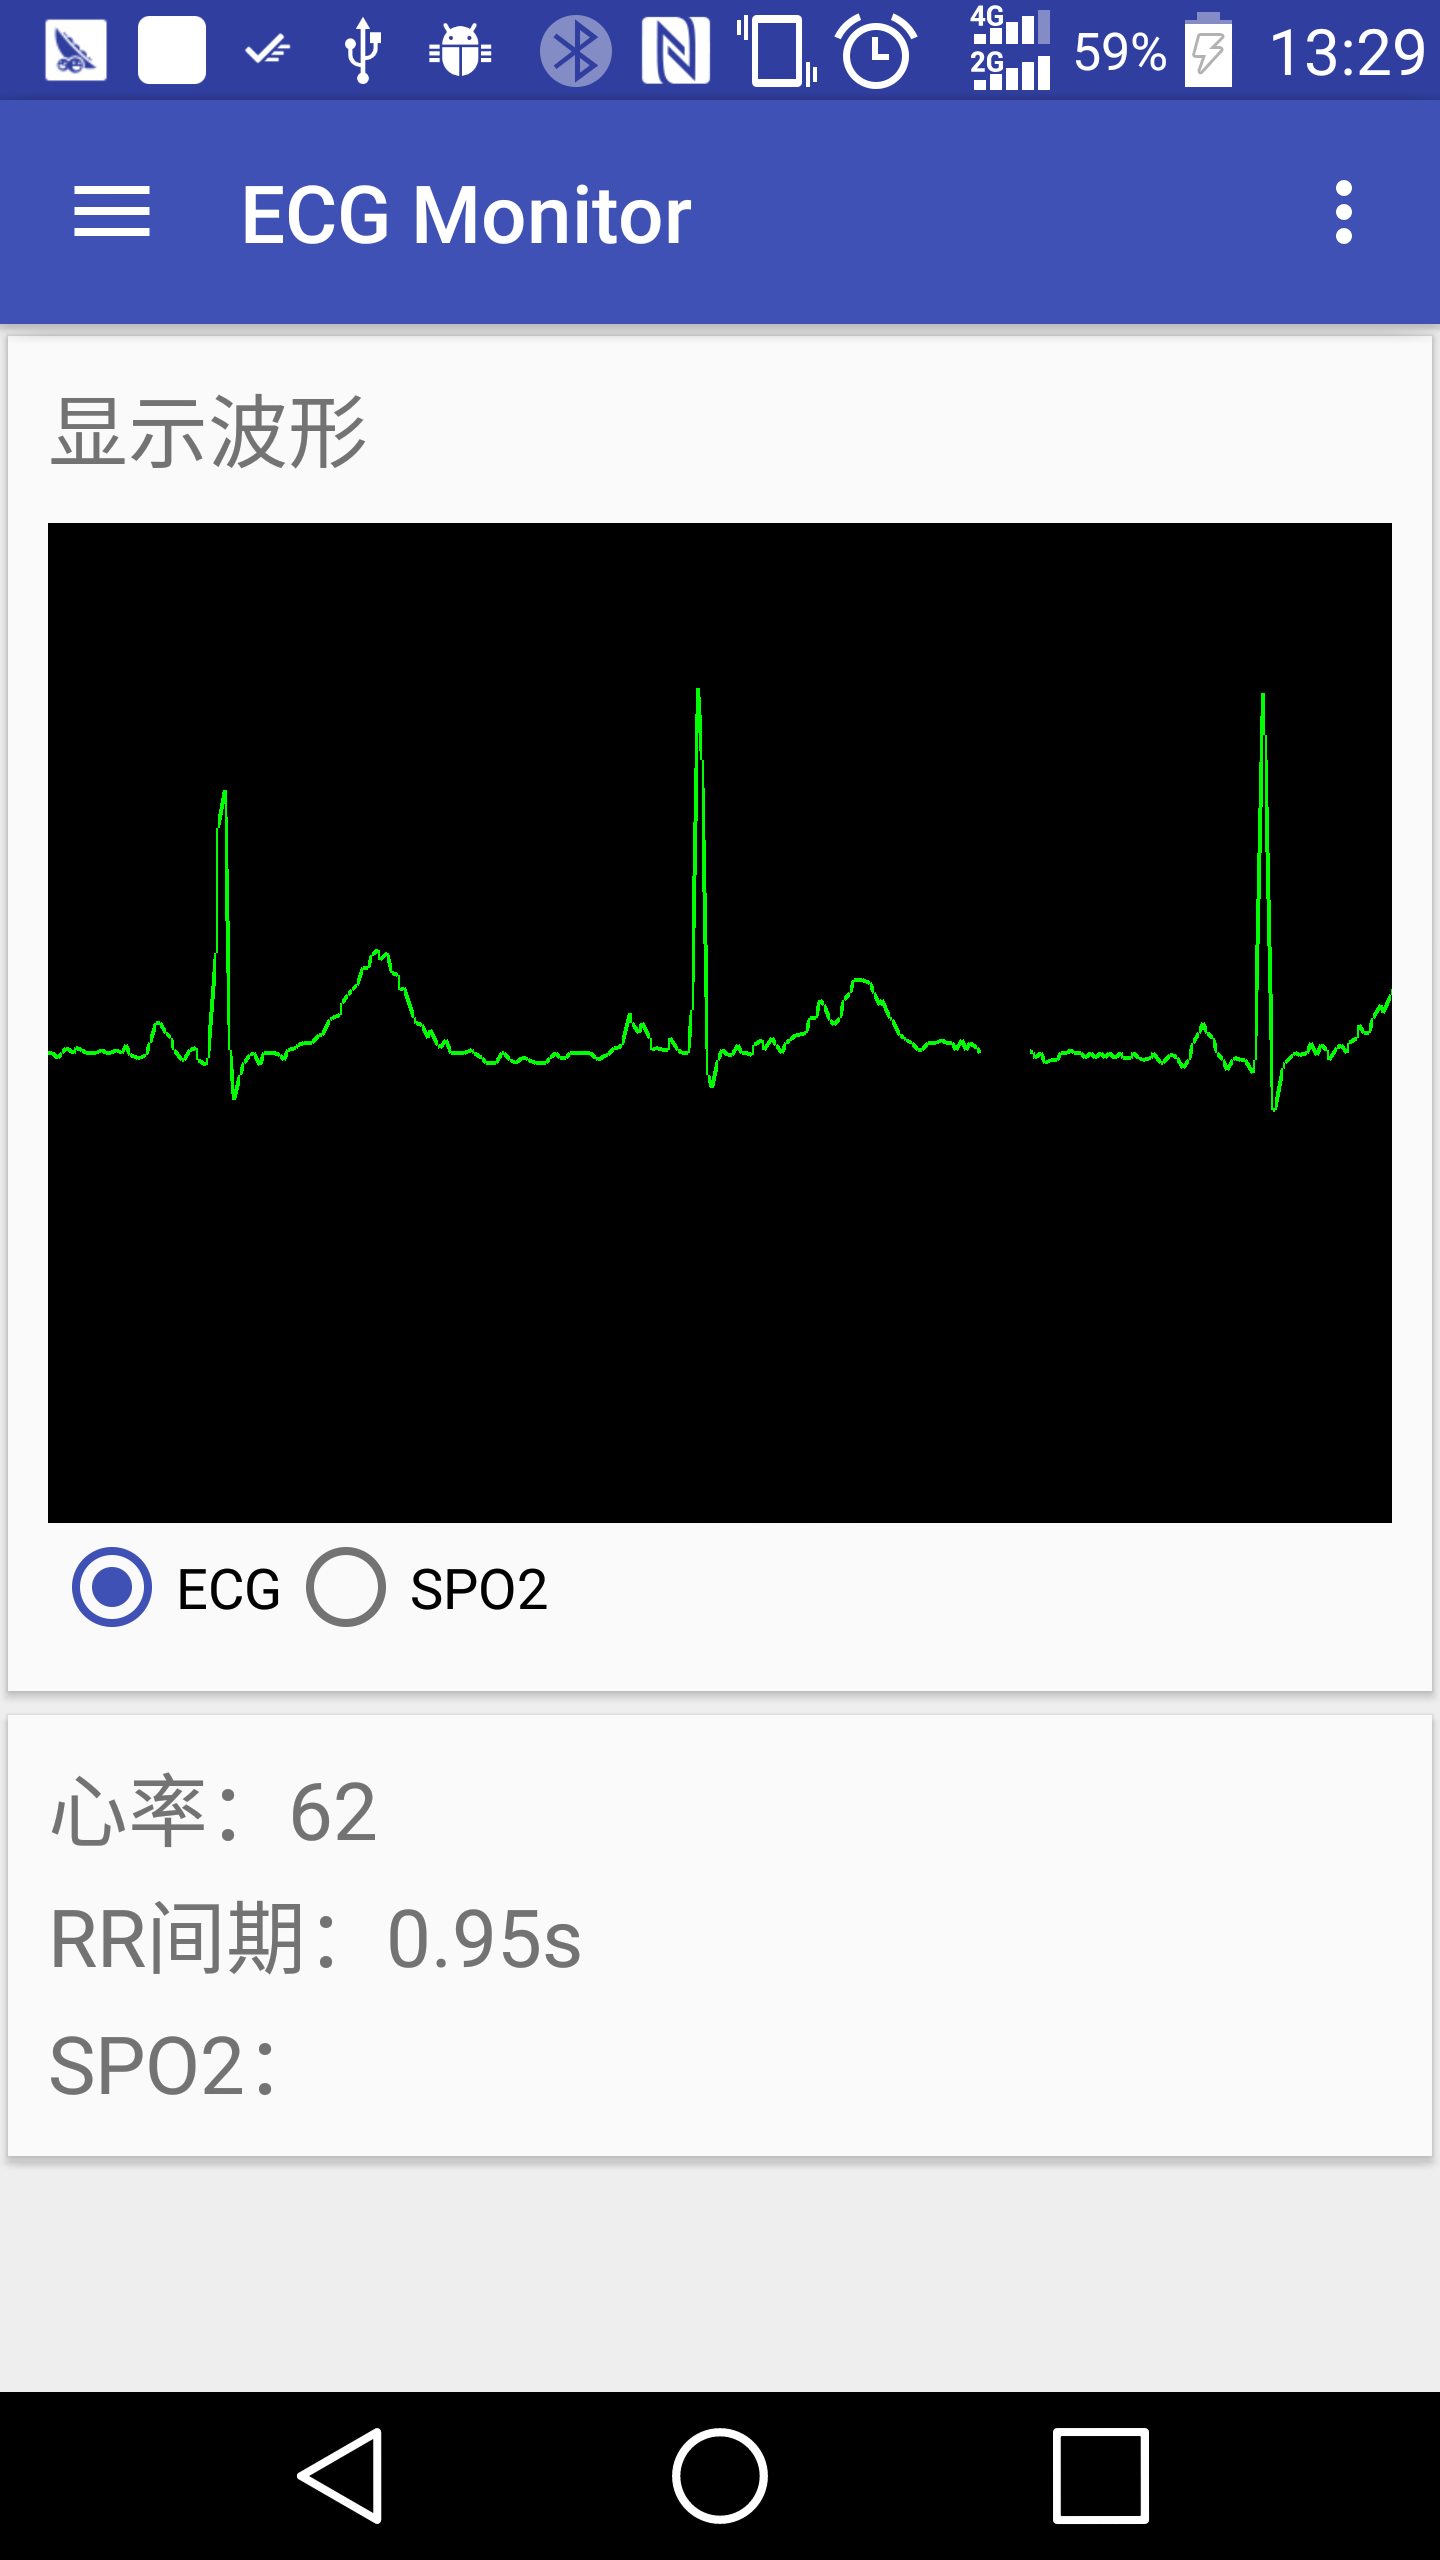
\includegraphics[height=6.8cm]{fig1.png}
			\end{center}
			\end{figure}}
			\only<2>
			{\begin{figure}[ht]
			\begin{center}
				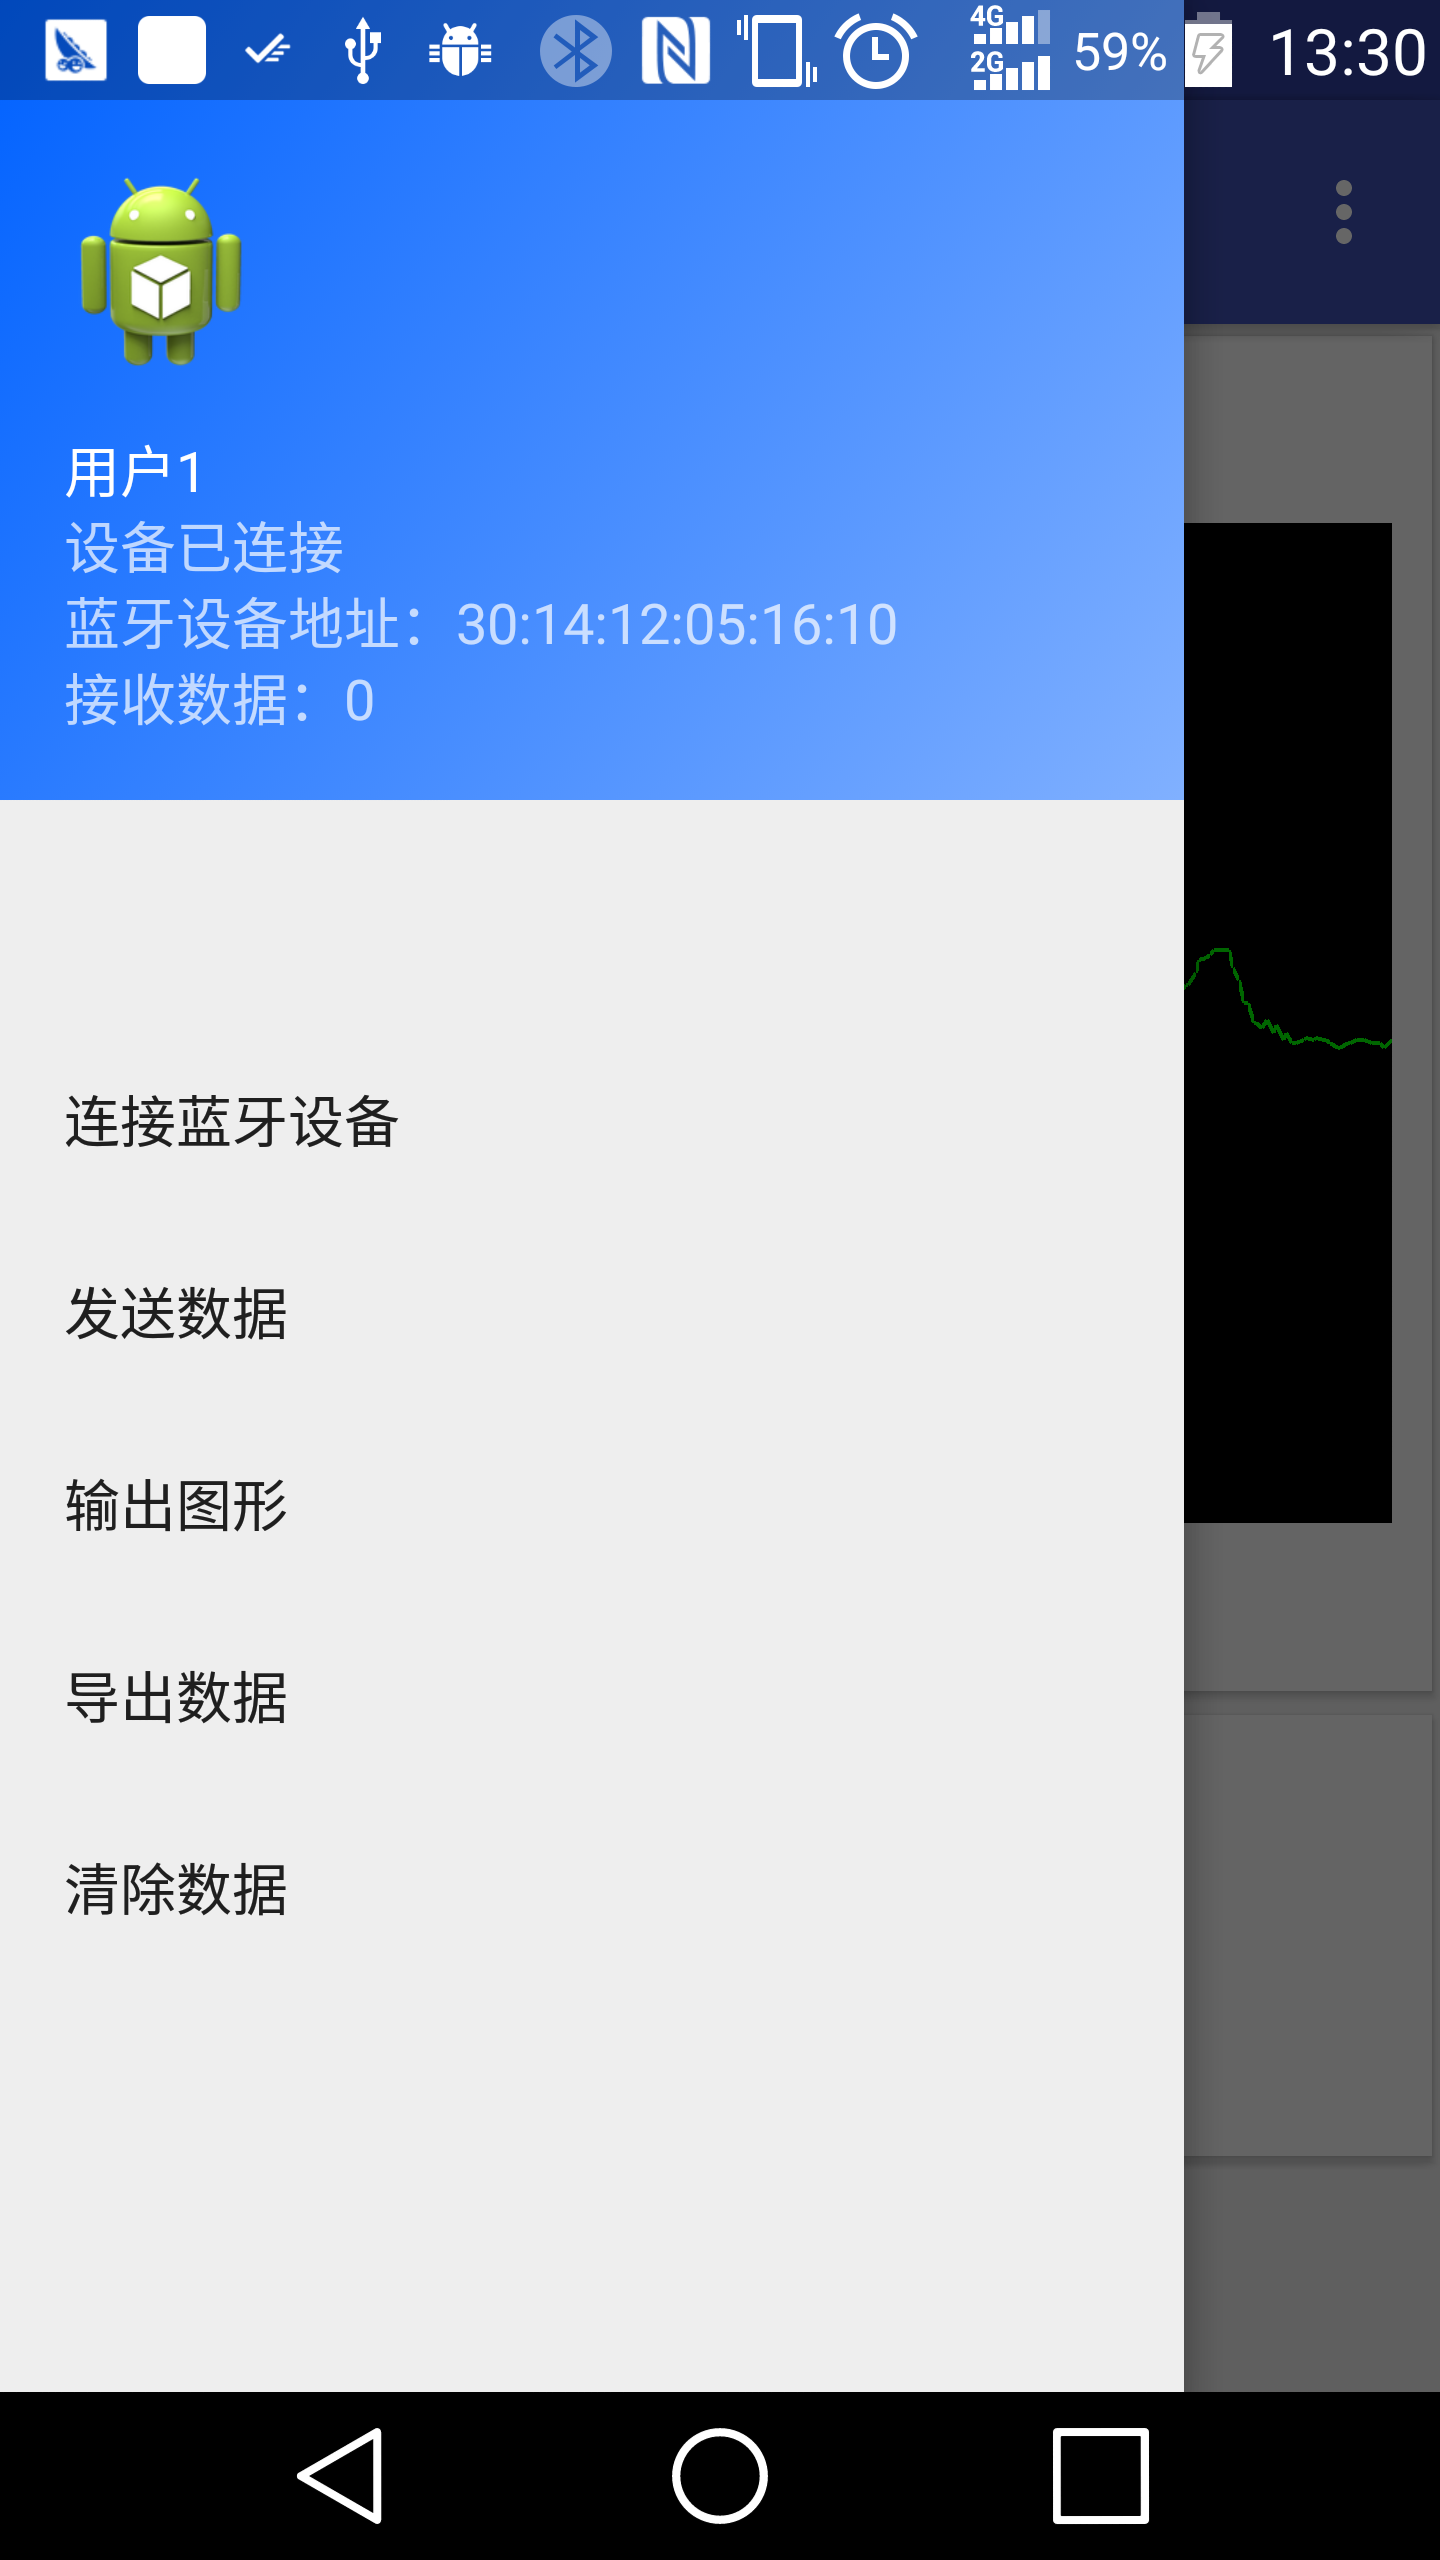
\includegraphics[height=6.8cm]{fig2.png}
			\end{center}
			\end{figure}}
		\column{0.5\textwidth}
			\begin{block}{显示方法的改进}
				显示方式适应设备的放置方式:横屏代表了详细的数据,竖屏代表了详细的操作
			\end{block}
			\only<1>
			{\begin{block}{}
				竖向屏幕包含了波形的简要显示
			\end{block}}
			\only<2>
			{\begin{block}{}
				菜单栏提供了更多选项和操作
			\end{block}}
	\end{columns}
\end{frame}

\begin{frame}{研究成果}{适应波形 可交互的显示方法}
	\begin{figure}[ht]
		\begin{center}
			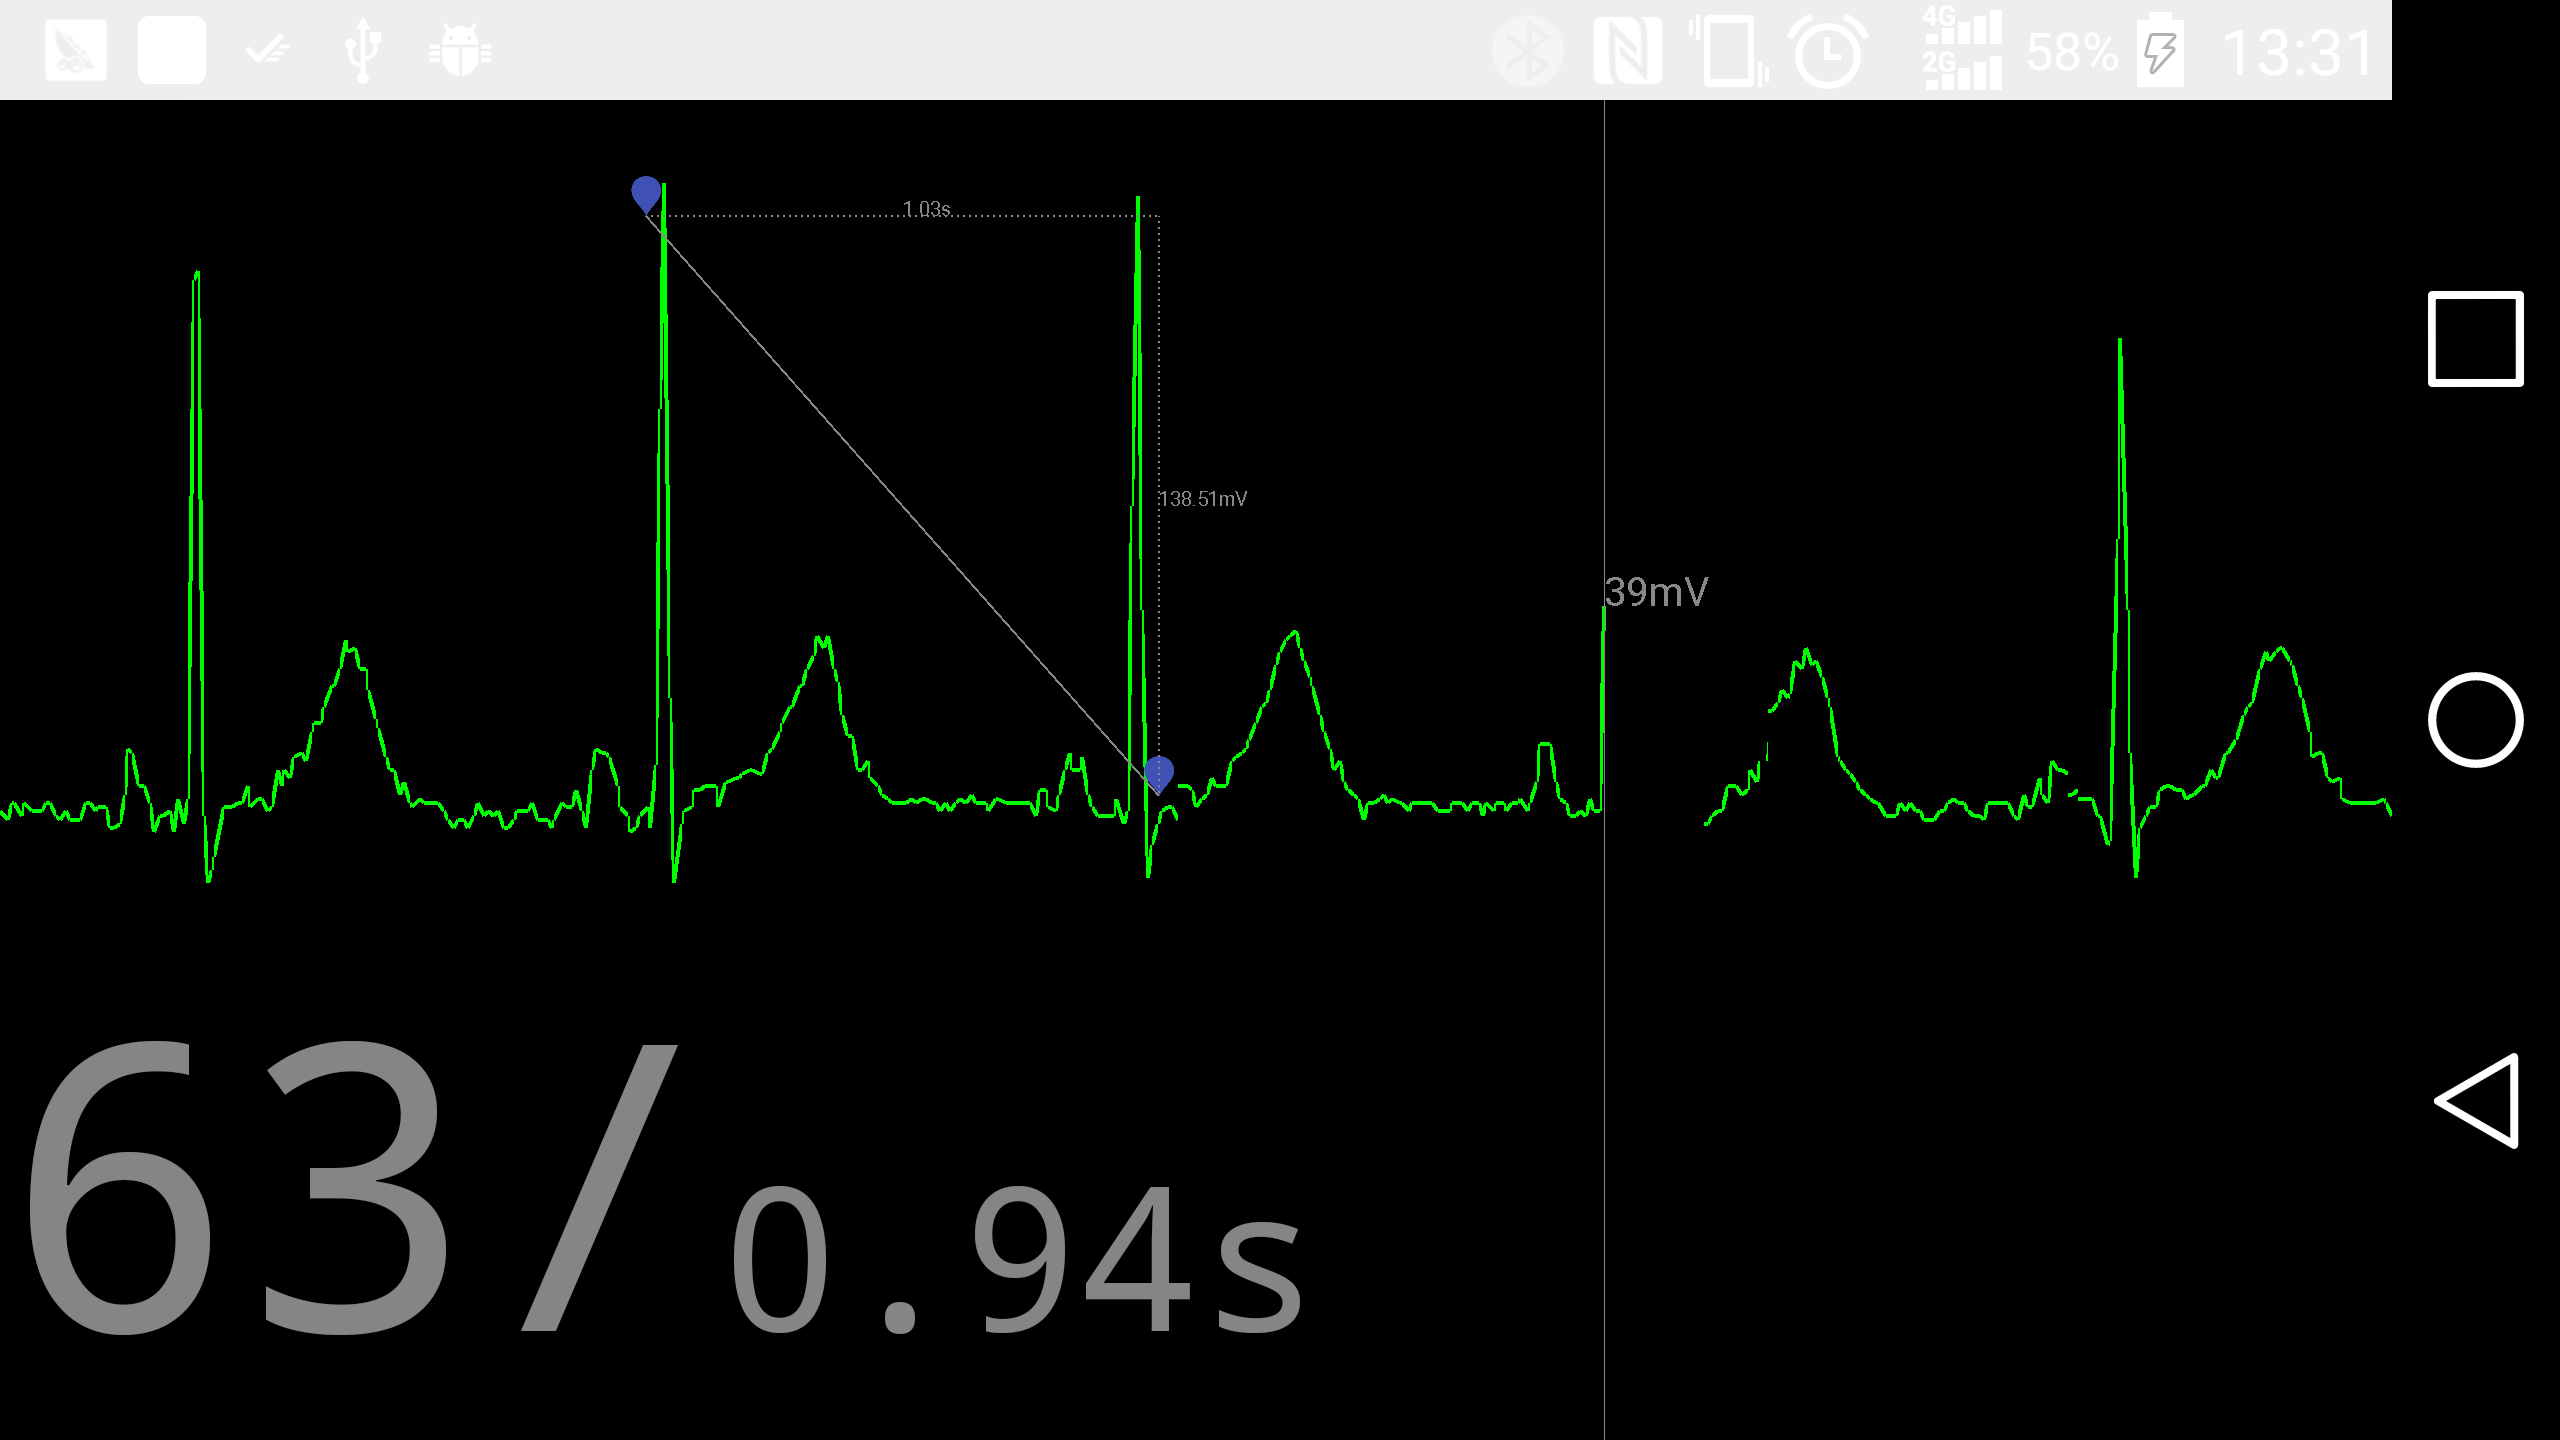
\includegraphics[height=4cm]{fig3.png}
		\end{center}
	\end{figure}
	\begin{block}{显示方法的改进}
		横向屏幕提供了波形的细节和测量波形的交互方式
	\end{block}
\end{frame}

\subsection{R峰检测算法}
\begin{frame}{研究成果}{高效准确的R峰检测算法}
	\begin{block}{滑动窗口最大值的R峰检测}
		\begin{itemize}
			\item 通过滑动窗口取最大值,检测R峰的出现。
			\item 算法复杂度小
			\item Se=99.7\%, Ac=99.7\%
		\end{itemize}
	\end{block}
\end{frame}

\section{应用实现}
\begin{frame}{应用实现}{应用架构设计}
\begin{columns}
\column{0.6\textwidth}
\begin{figure}[ht]
	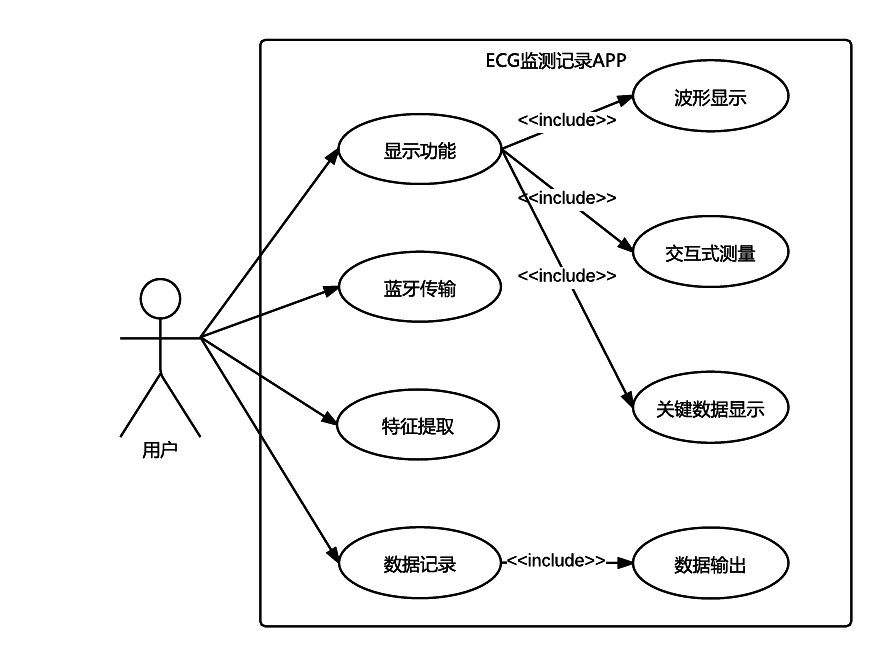
\includegraphics[width=\textwidth]{fig4.png}
\end{figure}
\column{0.4\textwidth}
\begin{block}{根据分析应用由以下组成:}
\begin{itemize}
	\item 显示模块
	\item 蓝牙传输模块 
	\item 数据库管理模块
	\item 数据分析模块
\end{itemize}
\end{block}
\end{columns}
\end{frame}

\subsection{显示模块}
\begin{frame}{应用实现}{显示模块的设计与实现}
\only<1>
{\begin{figure}[ht]
	\begin{center}
		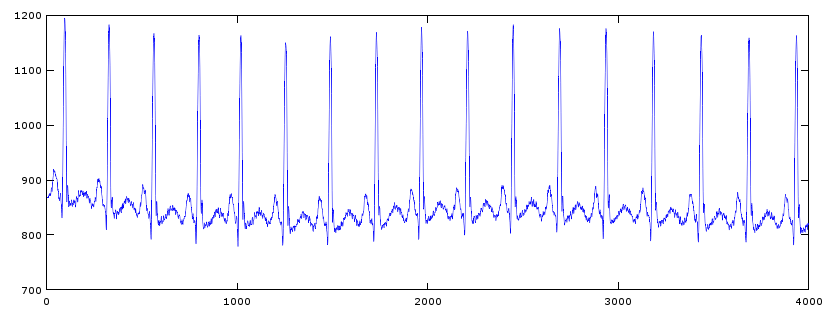
\includegraphics[width=\textwidth]{fig4-1a.png}
	\end{center}
\end{figure}}
\only<2>
{\begin{figure}
	\begin{center}
		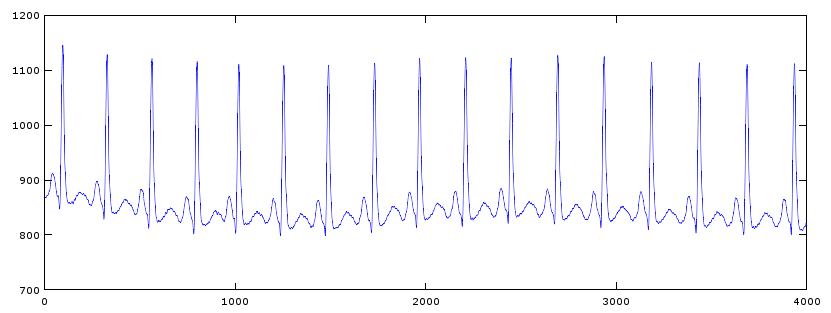
\includegraphics[width=\textwidth]{fig4-1b.png}
	\end{center}
\end{figure}}
\end{frame}

\begin{frame}[fragile]{应用实现}{显示模块的设计与实现}
\begin{block}{设置计时器完成采样工作}
\begin{center}
\begin{lstlisting}[language=java]
public DrawSurfaceView() { 
    x = 1; 
    shouldRefresh = false;
    setTimer(50);
} 
...
public void drawPoint(int drawX, int drawY) { 
    if (shouldRefresh) { 
        calculateXandY(x,y);
        shouldRefresh = false; 
        drawThread = new DrawThread(); 
        drawThread.start(); 
    } 
}
\end{lstlisting}
\end{center}
\end{block}
\end{frame}

\begin{frame}{应用实现}{显示模块的设计与实现}
\begin{figure}[ht]
	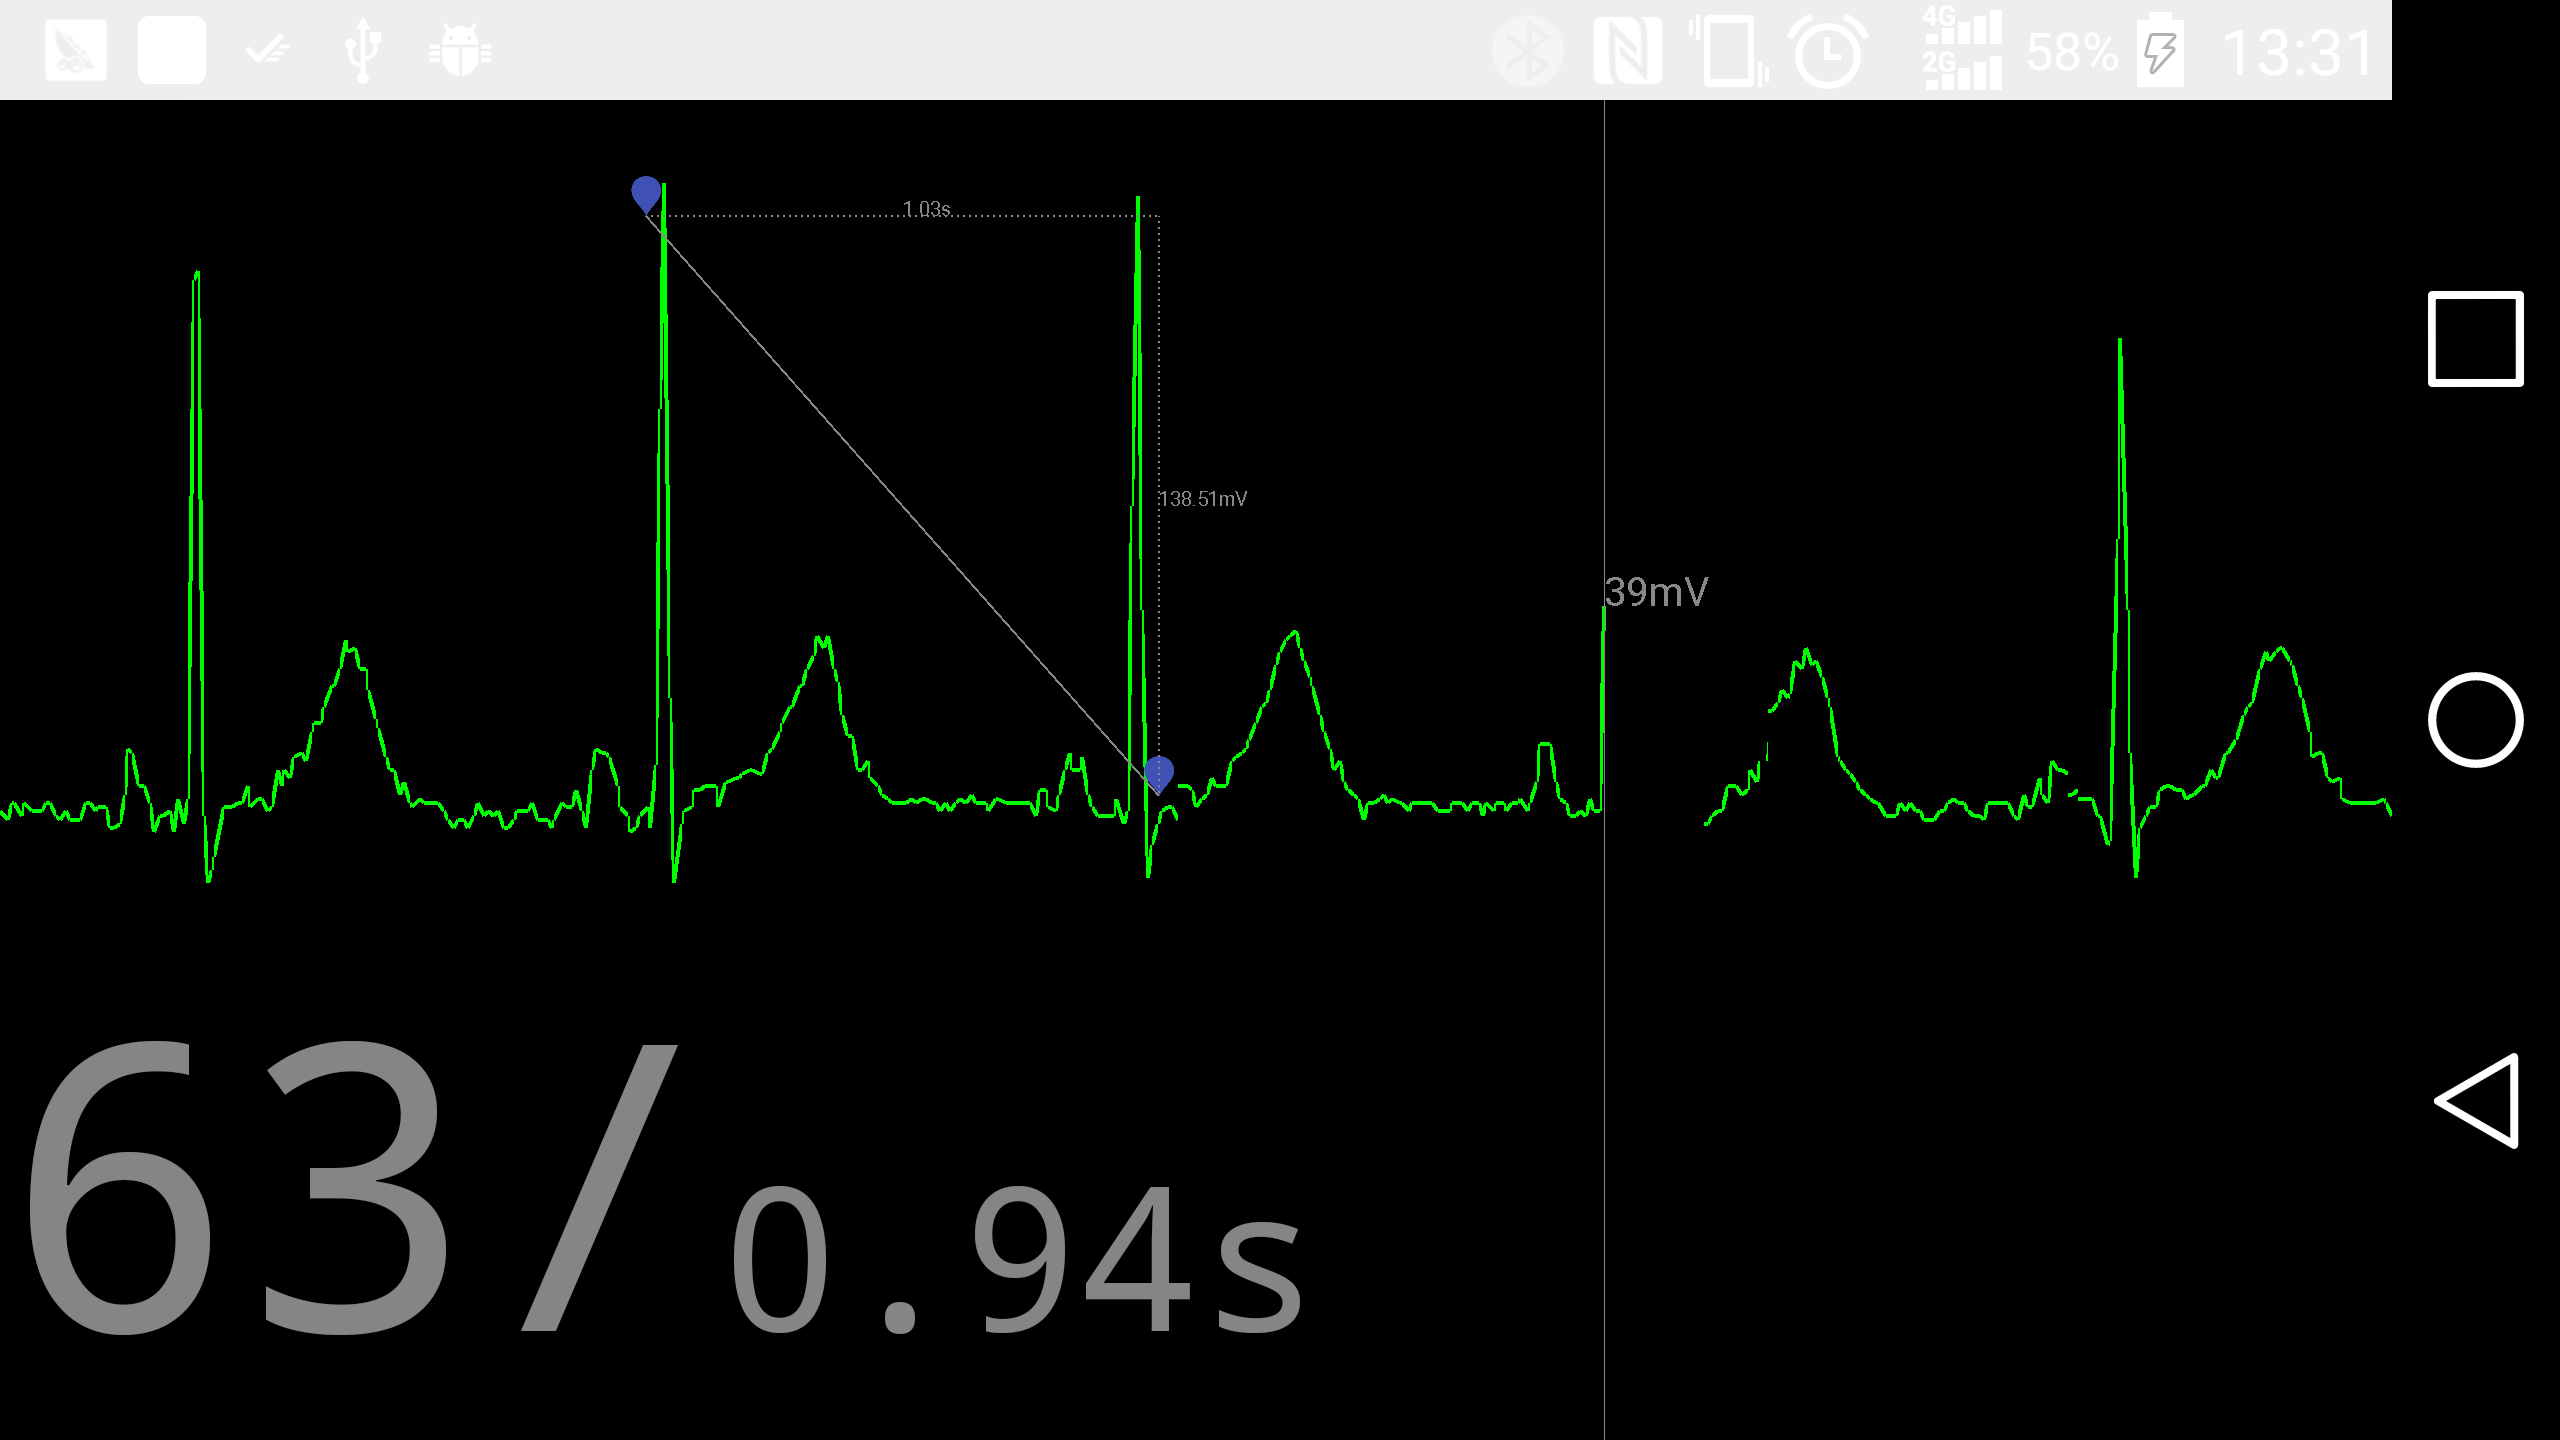
\includegraphics[width=\textwidth]{fig3.png}
\end{figure}
\end{frame}

\subsection{蓝牙传输模块}
\begin{frame}{应用实现}{蓝牙传输模块的设计与实现}
\begin{figure}[ht]
	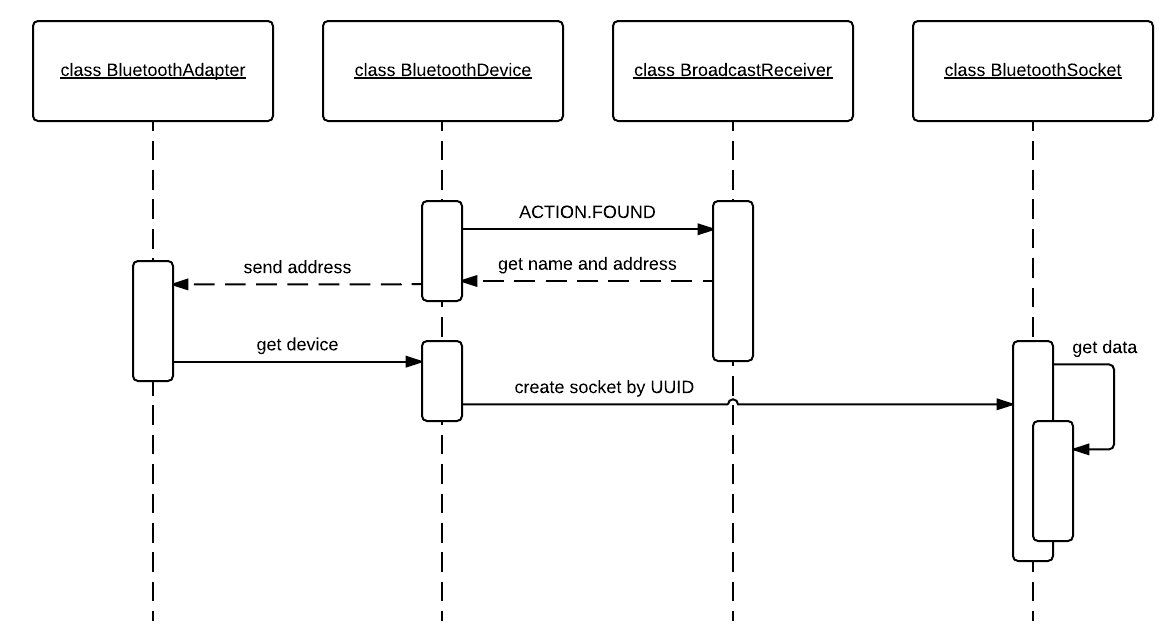
\includegraphics[width=\textwidth]{fig6.png}
	\caption{\label{fig1}蓝牙模块运行的UML时序图}
\end{figure}
\end{frame}

\subsection{数据库管理模块}
\begin{frame}{应用实现}{数据库管理模块的设计与实现}
\begin{columns}
\column{0.4\textwidth}
	\begin{figure}[ht]
		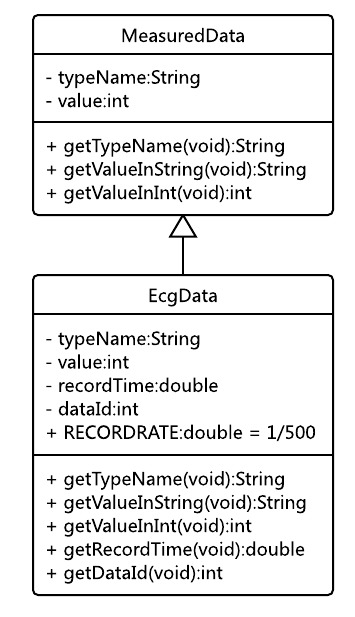
\includegraphics[width=\textwidth]{fig5.png}
	\end{figure}
\column{0.6\textwidth}
	\begin{block}{传输数据的格式化}
		\begin{itemize}
			\item 高程度抽象:MeasuredData父类作为所有收取数据的基础;
			\item 精准的时间戳:构造函数中计算时间,减少系统时间带来的误差;
			\item 时间戳的插入方法:随数据的实例化而自动插入;
			\item 各项属性的输出格式:提供多种格式的输出;
			\item 安全设计:数据属性外部无法访问;
		\end{itemize}
	\end{block}
\end{columns}
\end{frame}

\begin{frame}[fragile]{应用实现}{数据库管理模块的设计与实现}
\begin{block}{将多次数据插入操作作为一次事务提交}
\begin{center}
\begin{lstlisting}[language=java]
ecgDatabase.beginTransaction();
try {
    for (int cnt = 0; cnt < 500; cnt++) {
        insertData();
    }
    ecgDatabase.setTransactionSuccessful();
} finally {
    ecgDatabase.endTransaction();
    ecgDataTemp[0] = newEcgData;
}
\end{lstlisting}
\end{center}
\end{block}
\end{frame}

\subsection{数据分析模块}
\begin{frame}{应用实现}{数据分析模块的设计与实现}
\begin{block}{数据分析过程}<1->
EcgDataAnalyzer类通过滑动窗口(长度80)分批处理数据
\end{block}
\begin{block}{多线程并发访问的保护}<2->
专用于缓存的数据类型DataTemp中的属性访问函数均被synchronized,防止并发访问
\end{block}
\end{frame}

\section{算法实现}
\subsection{滑动窗口最大值算法}
\begin{frame}{算法实现}{基于滑动窗口的最大值算法检测R峰峰值}
\begin{block}{算法的检测步骤}
\begin{enumerate}
	\item<1-> 预处理:平均滤波器
	\item<2-> 取最大值,移动窗口
	\item<3-> 探测第一次R峰出现
	\item<4-> 根据第一次R峰检测剩余R峰
\end{enumerate}
\end{block}
\only<1>
{\begin{equation*}
  {{e}_{avg}}[j-5]=\frac{\sum\limits_{j=6}^{n}{e[j-5]+e[j-4]+,\ldots ,+e[j+4]}}{10}
\end{equation*}}
\only<2>
{\begin{equation*}
\begin{aligned}
 & {{t}_{\max }}=\max ({{e}_{\max }}[i],{{e}_{\max }}[i-1]); \\ 
 & {{t}_{avg}}={\sum\limits_{i=0}^{79}{{{e}_{avg}}[j+i]}}/{80}\;  
\end{aligned}
\end{equation*}}
\only<3>
{\begin{equation*}
\frac{{{t}_{\max }}}{{{t}_{avg}}}>1.2
\end{equation*}}
\only<4>
{\begin{equation*}
\left| \frac{{{t}_{\max }}-{{t}_{avg}}}{{{l}_{\max }}-{{l}_{avg}}}-1 \right|<0.5
\end{equation*}}
\end{frame}

\begin{frame}{算法实现}{基于滑动窗口的最大值算法检测R峰峰值}
\begin{figure}[ht]
	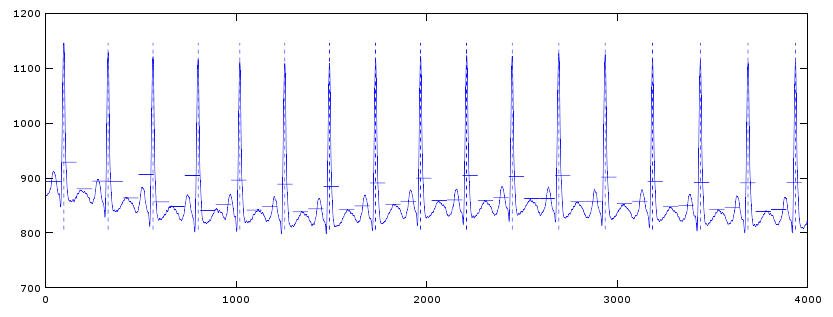
\includegraphics[width=\textwidth]{fig7.png}
\end{figure}
\end{frame}

\subsection{算法的Java实现}
\begin{frame}[fragile]{算法实现}{滑动窗口最大值算法的Java实现}
\begin{block}{求取最大值和平均数的同步运行}
\begin{center}
\begin{lstlisting}[language=java]
for (cnt = 0; cnt < 80; cnt++) {
    dataAvgValue += dataTemp[cnt].getData();
    if (rpeakLocalMax.getData() < dataTemp[cnt].getData()) {
        rpeakLocalMax = dataTemp[cnt];
    }
}
dataAvgValue = dataAvgValue / 80;
\end{lstlisting}
\end{center}
\end{block}
\end{frame}

\begin{frame}[fragile]{算法实现}{滑动窗口最大值算法的Java实现}
\begin{block}{数值向主线程的传递}
\begin{center}
\begin{lstlisting}[language=java]
double RRinterval = (recentRpeak.getDataId() -lastRpeak.getDataId()) * EcgData.RECORDRATE;
beatRate = 60 / RRinterval;
lastRpeak = recentRpeak;
Message uiRefreshMessage = Message.obtain();
uiRefreshMessage.what = 3;
uiRefreshMessage.arg1 = (int) beatRate;
uiRefreshMessage.arg2 = (int) (RRinterval*100);
uiRefreshHandler.sendMessage(uiRefreshMessage);
\end{lstlisting}
\end{center}
\end{block}
\end{frame}

\section{测试与结论}
\subsection{对R峰检测算法的测试}
\begin{frame}{测试与结论}{对R峰检测算法进行敏感度、准确度测试}
\begin{table}[htbp]
  \centering
  \caption{R峰检测算法的测试结果 % 表头
  \label{}}
  \liuhao
\begin{tabular}{|p{0.5cm}|p{0.4cm}|p{0.4cm}|p{0.4cm}|p{0.4cm}|p{0.4cm}|p{0.4cm}|p{0.4cm}|p{0.4cm}|p{0.4cm}|p{0.4cm}|p{0.5cm}|}
\hline 
数据 & 100 & 101 & 103 & 105 & 106 & 114 & 115 & 116 & 118 & 122 & 总计 \\ 
\hline 
TP & 74 & 71 & 70 & 82 & 66 & 54 & 63 & 79 & 71 & 87 & 717 \\ 
\hline 
FN & 0 & 0 & 0 & 1 & 0 & 0 & 0 & 0 & 1 & 0 & 2 \\ 
\hline 
Se(\%) & 100 & 100 & 100 & 98.8 & 100 & 100 & 100 & 100 & 98.6 & 100 & 99.7 \\ 
\hline 
Ac(\%) & 100 & 100 & 100 & 98.8 & 100 & 100 & 100 & 100 & 98.6 & 100 & 99.7 \\ 
\hline 
\end{tabular}  
\end{table}
\end{frame}

\subsection{应用程序的特点}
\begin{frame}{测试与结论}{ECG监测与记录应用的特点}
\begin{itemize}
\item 提出了适用于Android平台的ECG波形显示方法,能够更有效地显示波形;
\item 提出了能够与用户交互的波形测量方法,方便波形测量;
\item 提出了一种新的、适用于嵌入式平台的R峰检测算法,并且能够稳定、准确地检测R峰;
\item 实现了基于SQLite的ECG信号数据库,方便管理。
\end{itemize}
\end{frame}

%%%%%%%%%%%%%%%%%%%%end%%%%%%%%%%%%%%%%%%%%%%%%%%%%%%%
{\aauwavesbg
\begin{frame}[plain,noframenumbering]
  \finalpage{谢谢!}
\end{frame}}
\end{document}
